\chapter{Volume-Preserving SDOG Refinement} \label{chap:sdog}
One of the goals of this thesis is to produce 3D DGGS's with cells of as equal volume as possible.
The first approach we use for accomplishing this is modifying an existing 3D DGGS in order to improve its volume-preserving properties.
To this end, we chose to modify SDOG, as its use of a semiregular degenerate refinement means it already satisfies the primary goal of the thesis---that is, support for unbounded ranges of altitude.
The use of spherical coordinates also allows for efficient encoding and decoding operations, which we discuss in Chapter~\ref{chap:coding}.

The content of this chapter is taken from the article "Toward Volume Preserving Spheroid-Degenerated Octree Grid," authored by Benjamin Ulmer and Faramarz Samavati, which appeared in the journal \textit{Geoinformatica}~\cite{ulmer2020toward}.
Slight modifications have been made to maintain consistent terminology with the rest of the thesis, along with a more streamlined presentation of the methodology. Furthermore, the blending method presented in this chapter is different from the one that appears in the article.


\section{SDOG Overview} \label{chap:4:sdog}
Before describing our modifications, we first provide a brief explanation of SDOG construction and refinement as initially proposed by Yu and Wu~\cite{yu2009sdog}.
SDOG is an extension of the traditional octree to a spherical, as opposed to Euclidean, volume.
A sphere with twice the radius of the Earth is initially divided into eight equal octants via the equatorial plane and two perpendicular meridian planes.
These octants are taken to be the coarsest cells of the grid and are then refined to create more fine discretizations of the sphere.
Figure~\ref{fig:sdog} shows an SDOG octant after four applications of refinement.


\begin{figure}[ht!]
	\centering
	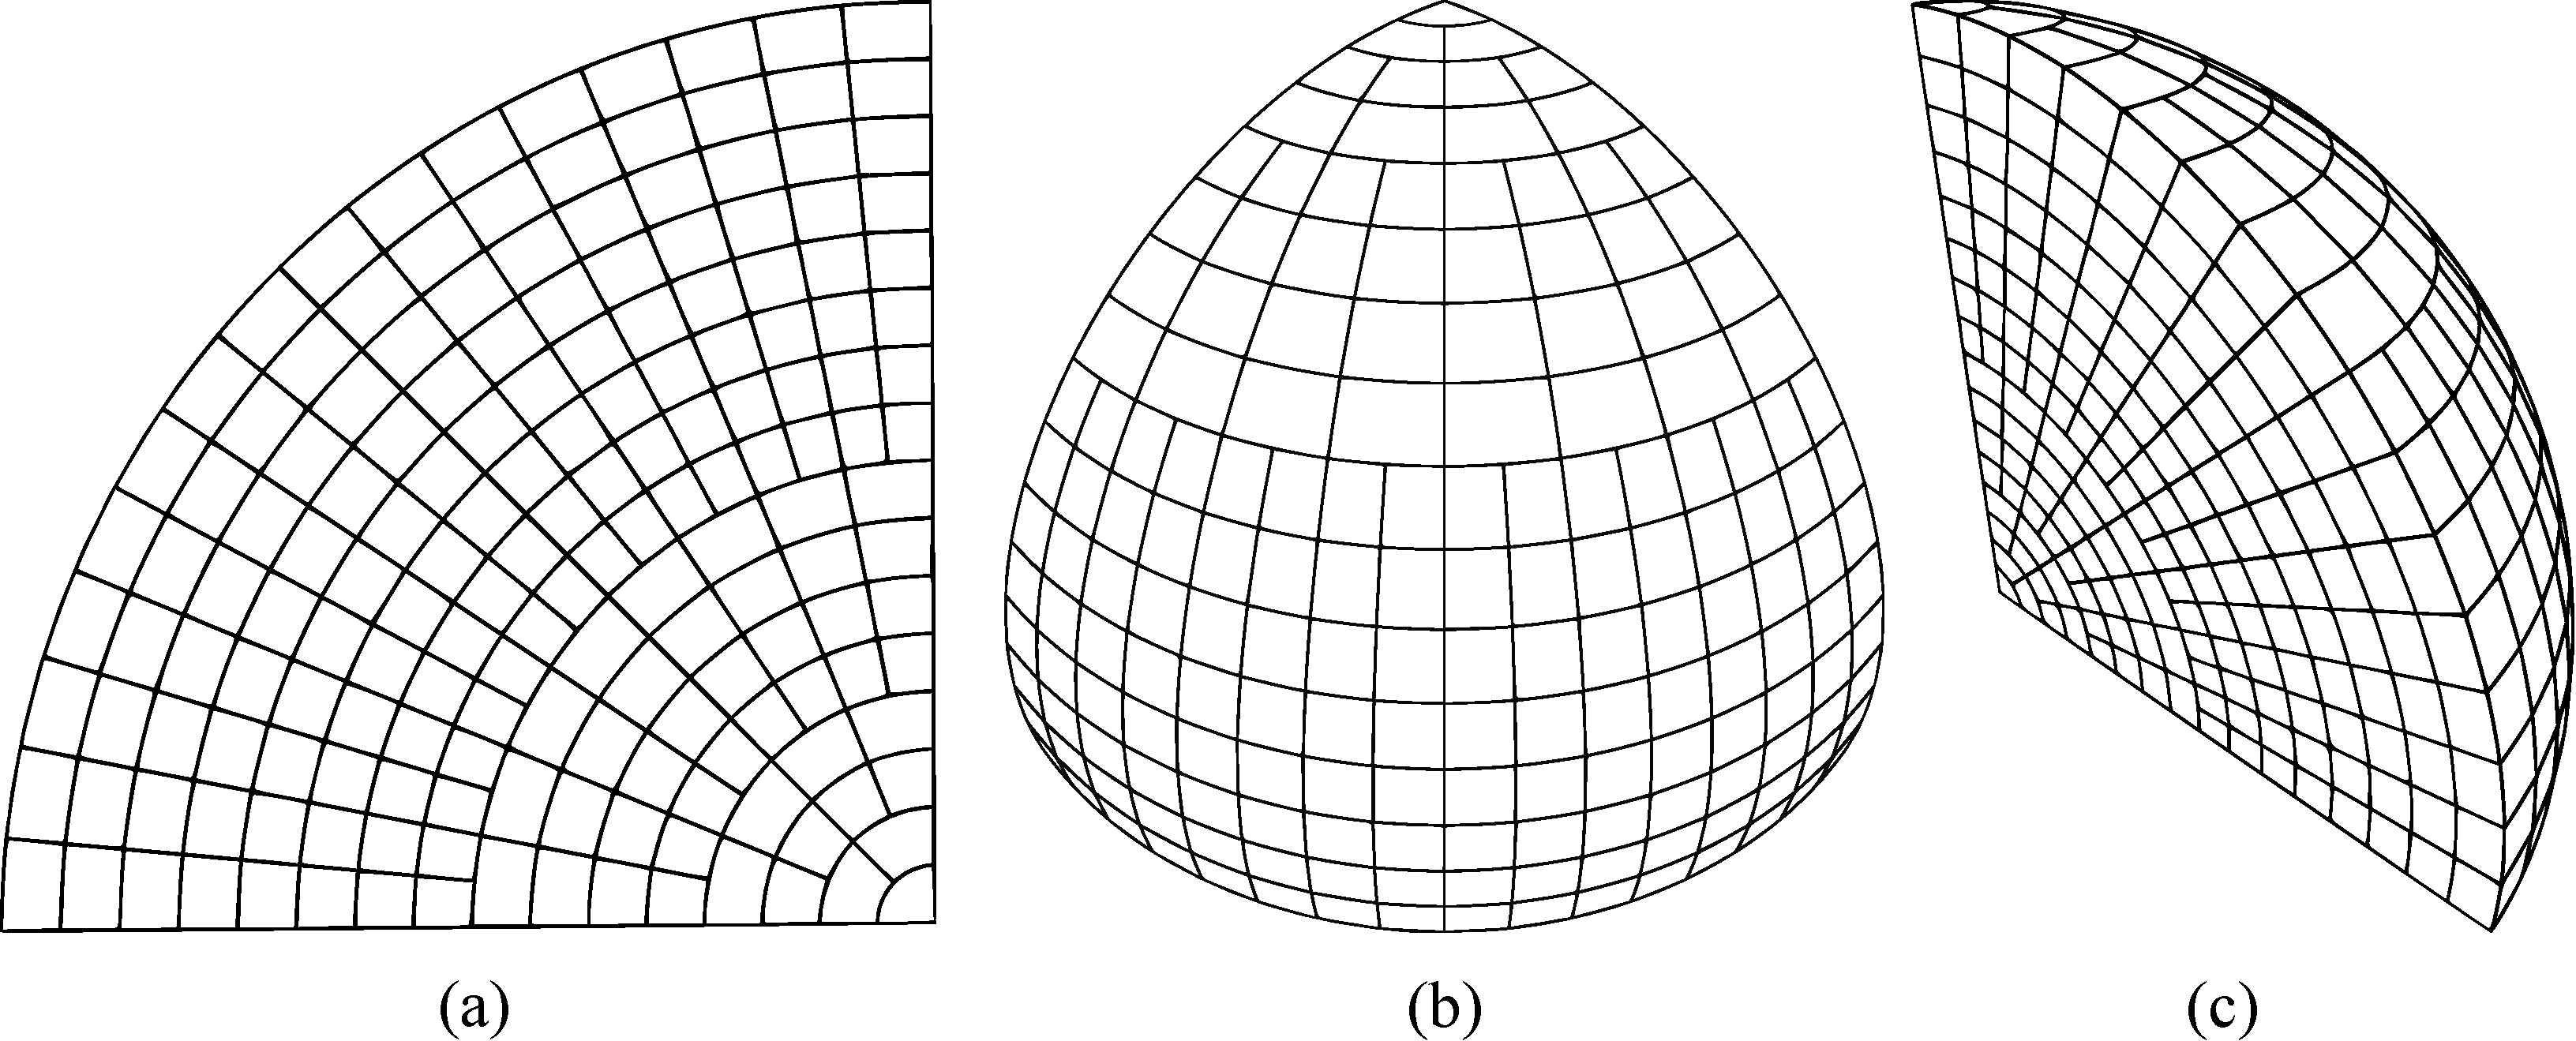
\includegraphics[width=\textwidth]{sdog.pdf}
	\caption[Title]{
		One octant of an SDOG grid after four levels of refinement viewed (a) from the side, (b) from the front, and (c) at an angle.
		Compared to a 3D LLG, cells are more uniform in size and have better compactness.
		Refer to Chapter~\ref{chap:4:results} for a detailed analysis of the volume and compactness properties of SDOG
	}
	\label{fig:sdog}
\end{figure}


\begin{figure}[ht!]
	\centering
	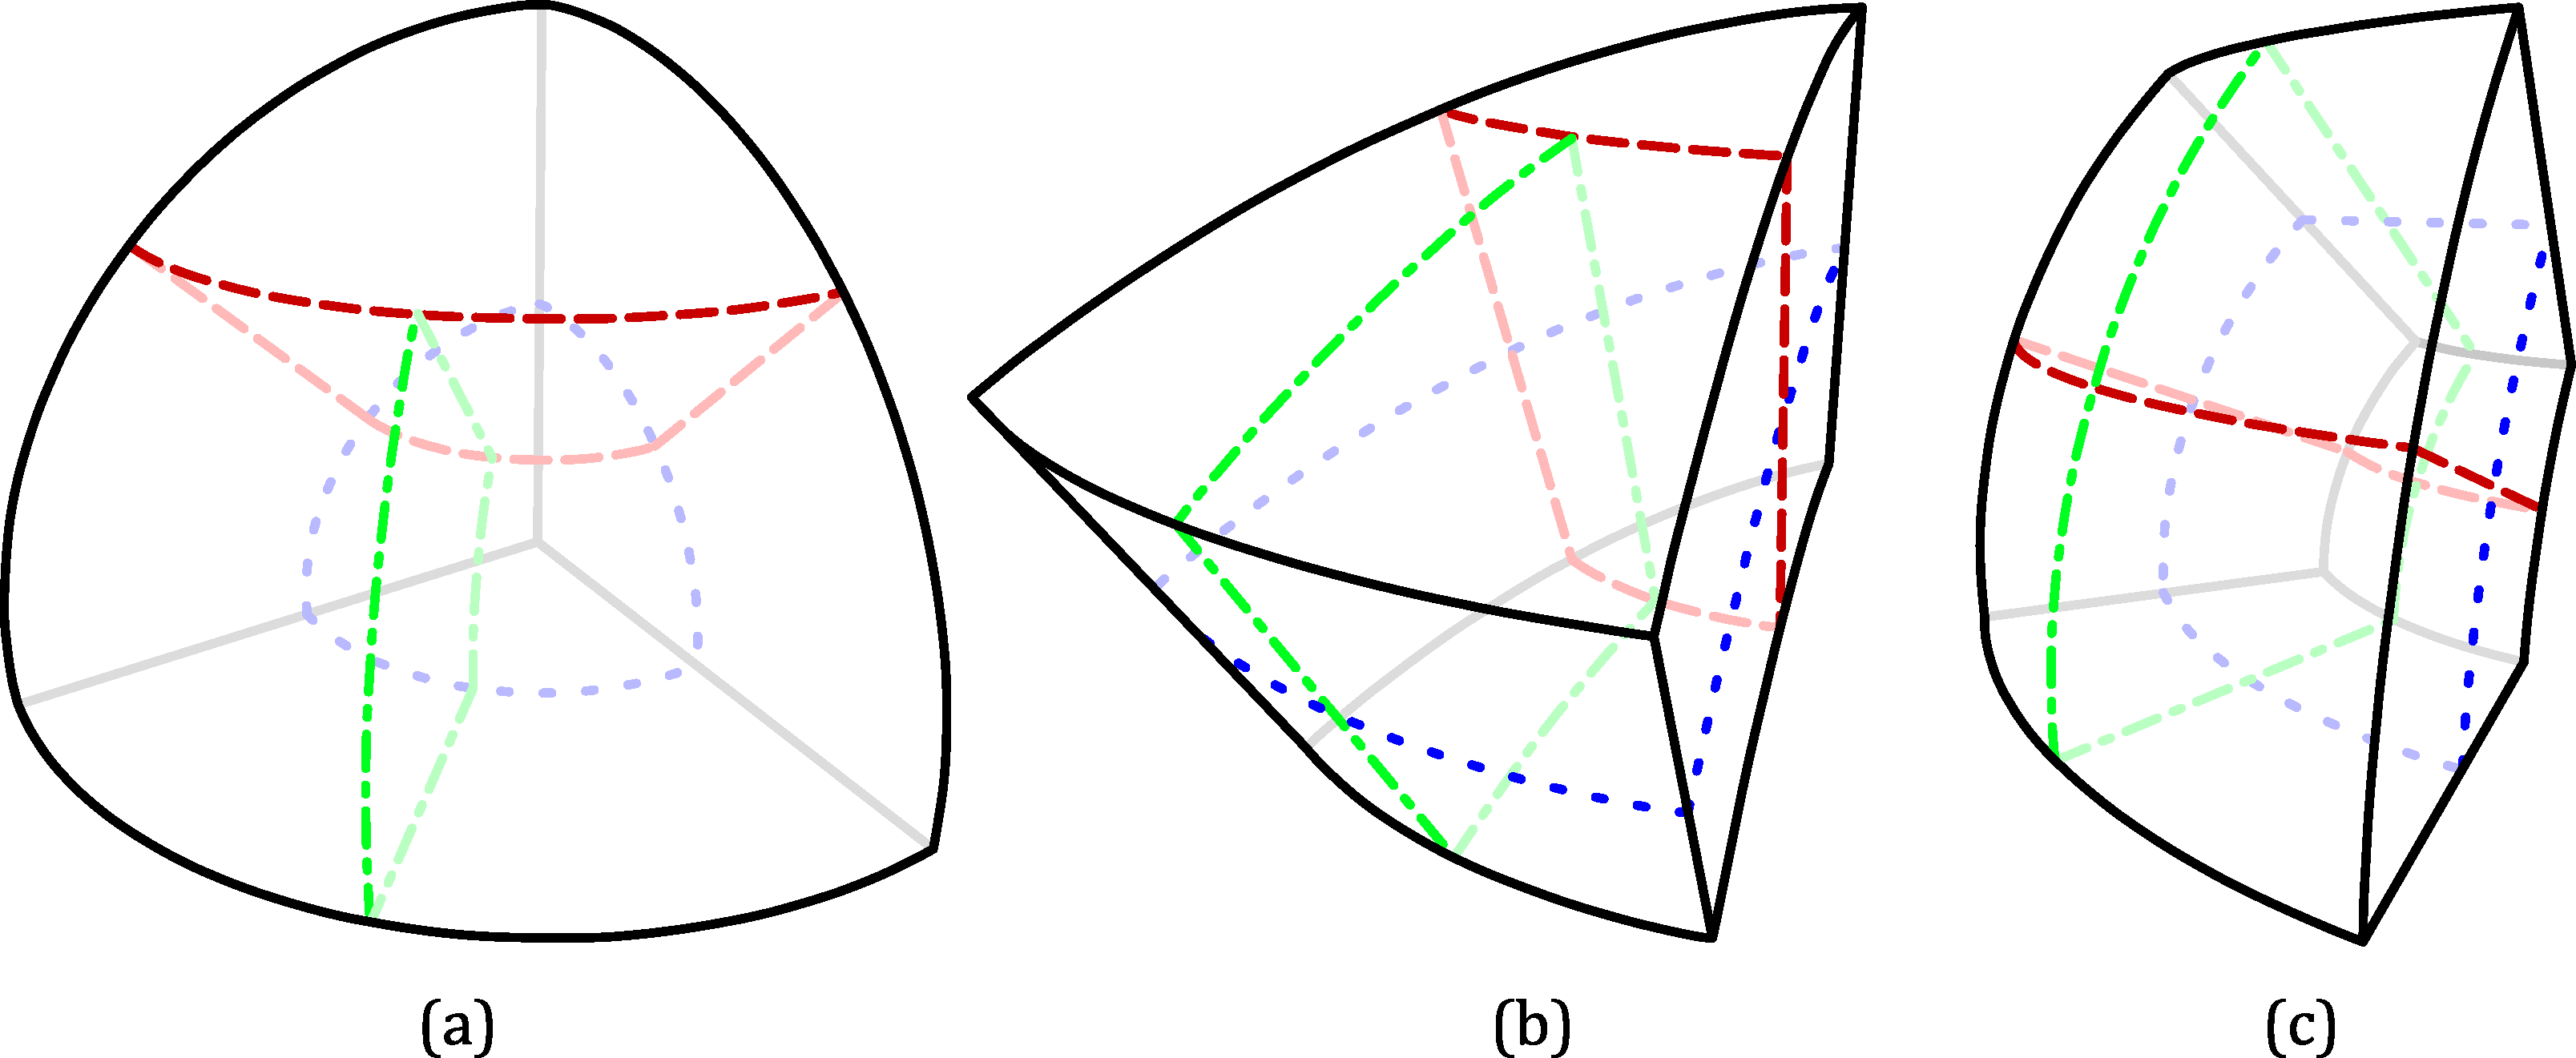
\includegraphics[width=\textwidth]{sdog-refinement.pdf}
	\caption[Title]{
		Location and extent of splitting surfaces in SDOG refinement for (a) SG cells, (b) LG cells, and (c) NG cells.
		Only NG cells have all three splitting surfaces fully refine the cell into eight children, and make up the majority of cells as the grid becomes increasingly refined
	}
	\label{fig:sdog-refinement}
\end{figure}


SDOG cells---including octants---are refined using the midpoint of each spherical coordinate: latitude, longitude, and radius.
These midpoints create splitting surfaces used to split parent cells into smaller children cells.
As described in Chapter~\ref{chap:3:semiregDegen}, a semiregular degenerate refinement is used to prevent excessive degeneration in cell size and compactness near the poles and centre of the sphere.
As a result, SDOG cells are grouped into three classes, depending on which singularities they border.
Figure~\ref{fig:sdog-refinement} shows the resulting splitting surfaces for each type of SDOG cell.
%We call a splitting surface symmetric if it creates the same number and type(s) of cells on both sides; otherwise we call it degenerate.


Cells that extend to the centre of the sphere and one of the poles are referred to as Sphere-degenerated Grid (SG) cells (Figure~\ref{fig:sdog-refinement}a) and include the original eight octants.
For these cells, the longitudinal splitting surface does not extend beyond the latitudinal one in the direction towards the pole.
Additionally, neither the latitudinal nor longitudinal splitting surfaces extend beyond the radial one in the direction towards the centre of the sphere.
The result of this refinement is four children cells: another SG cell, one Latitude-degenerated Grid (LG) cell, and two Normal Grid (NG) cells.
We describe LG and NG cells below.
%Only the longitudinal splitting surface for SG cells is symmetric.


LG cells (Figure~\ref{fig:sdog-refinement}b) are similar to SG ones, except that they only extend to one of the poles and not the centre of the sphere.
Therefore, the longitudinal splitting surface does not extend beyond the latitudinal one in the direction towards the pole.
This refinement results in six children cells: two LG cells and four NG cells.
%The longitudinal and radial splitting surfaces for LG cells are symmetric.


NG cells (Figure~\ref{fig:sdog-refinement}c) extend to neither the pole nor the centre of the sphere and make up the majority of SDOG cells.
These cells are fully refined into eight children NG cells and are the regular case for SDOG refinement.
%All splitting surfaces for NG cells are symmetric.


\subsection{Number of SDOG Cells} \label{chap:4:numCells}
Being able to analyze the number of cells in the grid at each level of refinement is useful not only for measuring volume-preserving properties---such as quickly calculating the average cell volume---but also for analyzing the behaviour of the grid as the level of refinement increases.
This type of analysis will prove useful in informing decisions about how to modify refinement to improve volume preservation.


Due to the degenerate nature of SDOG refinement, calculating the number of cells in the grid is more complicated than a simple exponential formulation.
Despite this, we can use the above refinement rules to derive recursive definitions for the number of cells in an SDOG grid (or a single octant) at a given level of refinement.
Let $S(k)$, $L(k)$, $N(k)$, and $T(k)$ be the number of SG, LG, NG, and total cells of an SDOG octant at refinement level $k$, respectively.
There is only ever one SG cell in an SDOG octant, so trivially
%
\begin{equation*}
S(k) = 1.
\end{equation*}
%
We know each LG cell produces two new LG cells, and that the SG cell produces one new LG cell.
From this we say
%
\begin{equation*}
L(k) = 2L(k-1) + 1 \quad\text{and}\quad L(1) = 1.
\end{equation*}
%
Similarly, each NG cell produces eight new NG cells, each LG cell produces four, and the SG cell produces two.
Thus
%
\begin{equation*}
N(k) = 8N(k-1) + 4L(k-1) + 2 \quad\text{and}\quad N(1) = 2.
\end{equation*}
%
$L(k)$ is a linear non-homogeneous recurrence which can be solved with standard techniques \cite{bellman1963differential}.
Solving and substituting into $N(k)$ we get another linear non-homogeneous recurrence which can be solved similarly.
Finally, we get the closed forms:
%
\begin{equation*}
L(k) = 2^{k} - 1,
\end{equation*}
%
\begin{equation*}
N(k) = \frac{1}{21} \left( 7*2^{k} + 8^{k+1} + 6 \right) - 2^{k}, \quad\text{and}
\end{equation*}
%
\begin{equation*}
T(k) = S(k) + L(k) + N(k) = \frac{1}{21} \left( 7*2^{k} + 8^{k+1} + 6 \right).
\end{equation*}
%
As far as we are aware, these formulations have not been provided in any of the preexisting literature on SDOG.


\subsection{Geometry of SDOG Cells} \label{chap:4:geom}
In order to measure the volume preservation properties of SDOG and its modifications, it is necessary to be able to measure the volume of individual cells in the grid.
Since each SDOG cell represents a range of each spherical coordinate (latitude $\phi$, longitude $\lambda$, and radius $r$), calculating the volume of an individual cell is a straightforward task.
Note that we use the geographic convention for spherical coordinates in this thesis.
Let the subscripts $\mathrm{max}$ and $\mathrm{min}$ denote the maximum and minimum of a given spherical coordinate for an SDOG cell; then, the volume is \cite{yu2009sdog}
%
\begin{equation} \label{eq:volume}
V = \frac{1}{3} \left( \lambda_\mathrm{max} - \lambda_\mathrm{min} \right) \left(r_\mathrm{max}^{3} - r_\mathrm{min}^{3} \right) \left(\sin\phi_\mathrm{max} - \sin\phi_\mathrm{min} \right).
\end{equation}


In addition to the volume of a cell, surface area is another useful property to be able to measure.
Combined with the volume of cells, this allows us to measure the compactness of cells, which we use in Chapter~\ref{chap:4:results} to help evaluate the consequences of our modifications.
From the fact that SDOG cells are refined using spherical coordinates, each face of a cell is a section of a simple geometric shape.
Faces created by radial splitting surfaces are spherical, with surface area given by
%
\begin{equation*}
r^2 \left( \lambda_\mathrm{max} - \lambda_\mathrm{min} \right) \left( \sin\phi_\mathrm{max} - \sin\phi_\mathrm{min} \right).
\end{equation*}
%
Faces created by longitudinal splitting surfaces are the difference of two circular sectors, and have an area of
%
\begin{equation*}
\frac{1}{2} \left( \phi_\mathrm{max} - \phi_\mathrm{min} \right) \left( r_\mathrm{max}^{2} - r_\mathrm{min}^{2} \right).
\end{equation*}
%
Finally, faces created by latitudinal splitting surfaces lie on a cone, with a surface area of
%
\begin{equation*}
\frac{1}{2} \cos\phi \left( \lambda_\mathrm{max} - \lambda_\mathrm{min} \right) \left( r_\mathrm{max}^{2} - r_\mathrm{min}^{2} \right).
\end{equation*}


\section{Modified SDOG Refinement} \label{chap:4:modified}
The main goal of this work is to modify SDOG in such a way as to improve volume preservation while minimizing the impact on other desired properties of the grid.
As a baseline, the distribution of cell volumes in a conventional SDOG grid is visualized in Figure~\ref{fig:sdog-volume}.
In conventional SDOG refinement, the location of the different splitting surfaces is always at the midpoint of the respective spherical coordinate; we question if this should be the case.
For an octree in Euclidean space, this type of refinement is desirable, as it generates children cells of identical size and shape.
In spherical space, however, this property does not transfer.
Using midpoints to refine cells makes for a simple refinement scheme, but it makes no guarantees about the shape or size of the resulting child cells.


\begin{figure}[ht!]
	\centering
	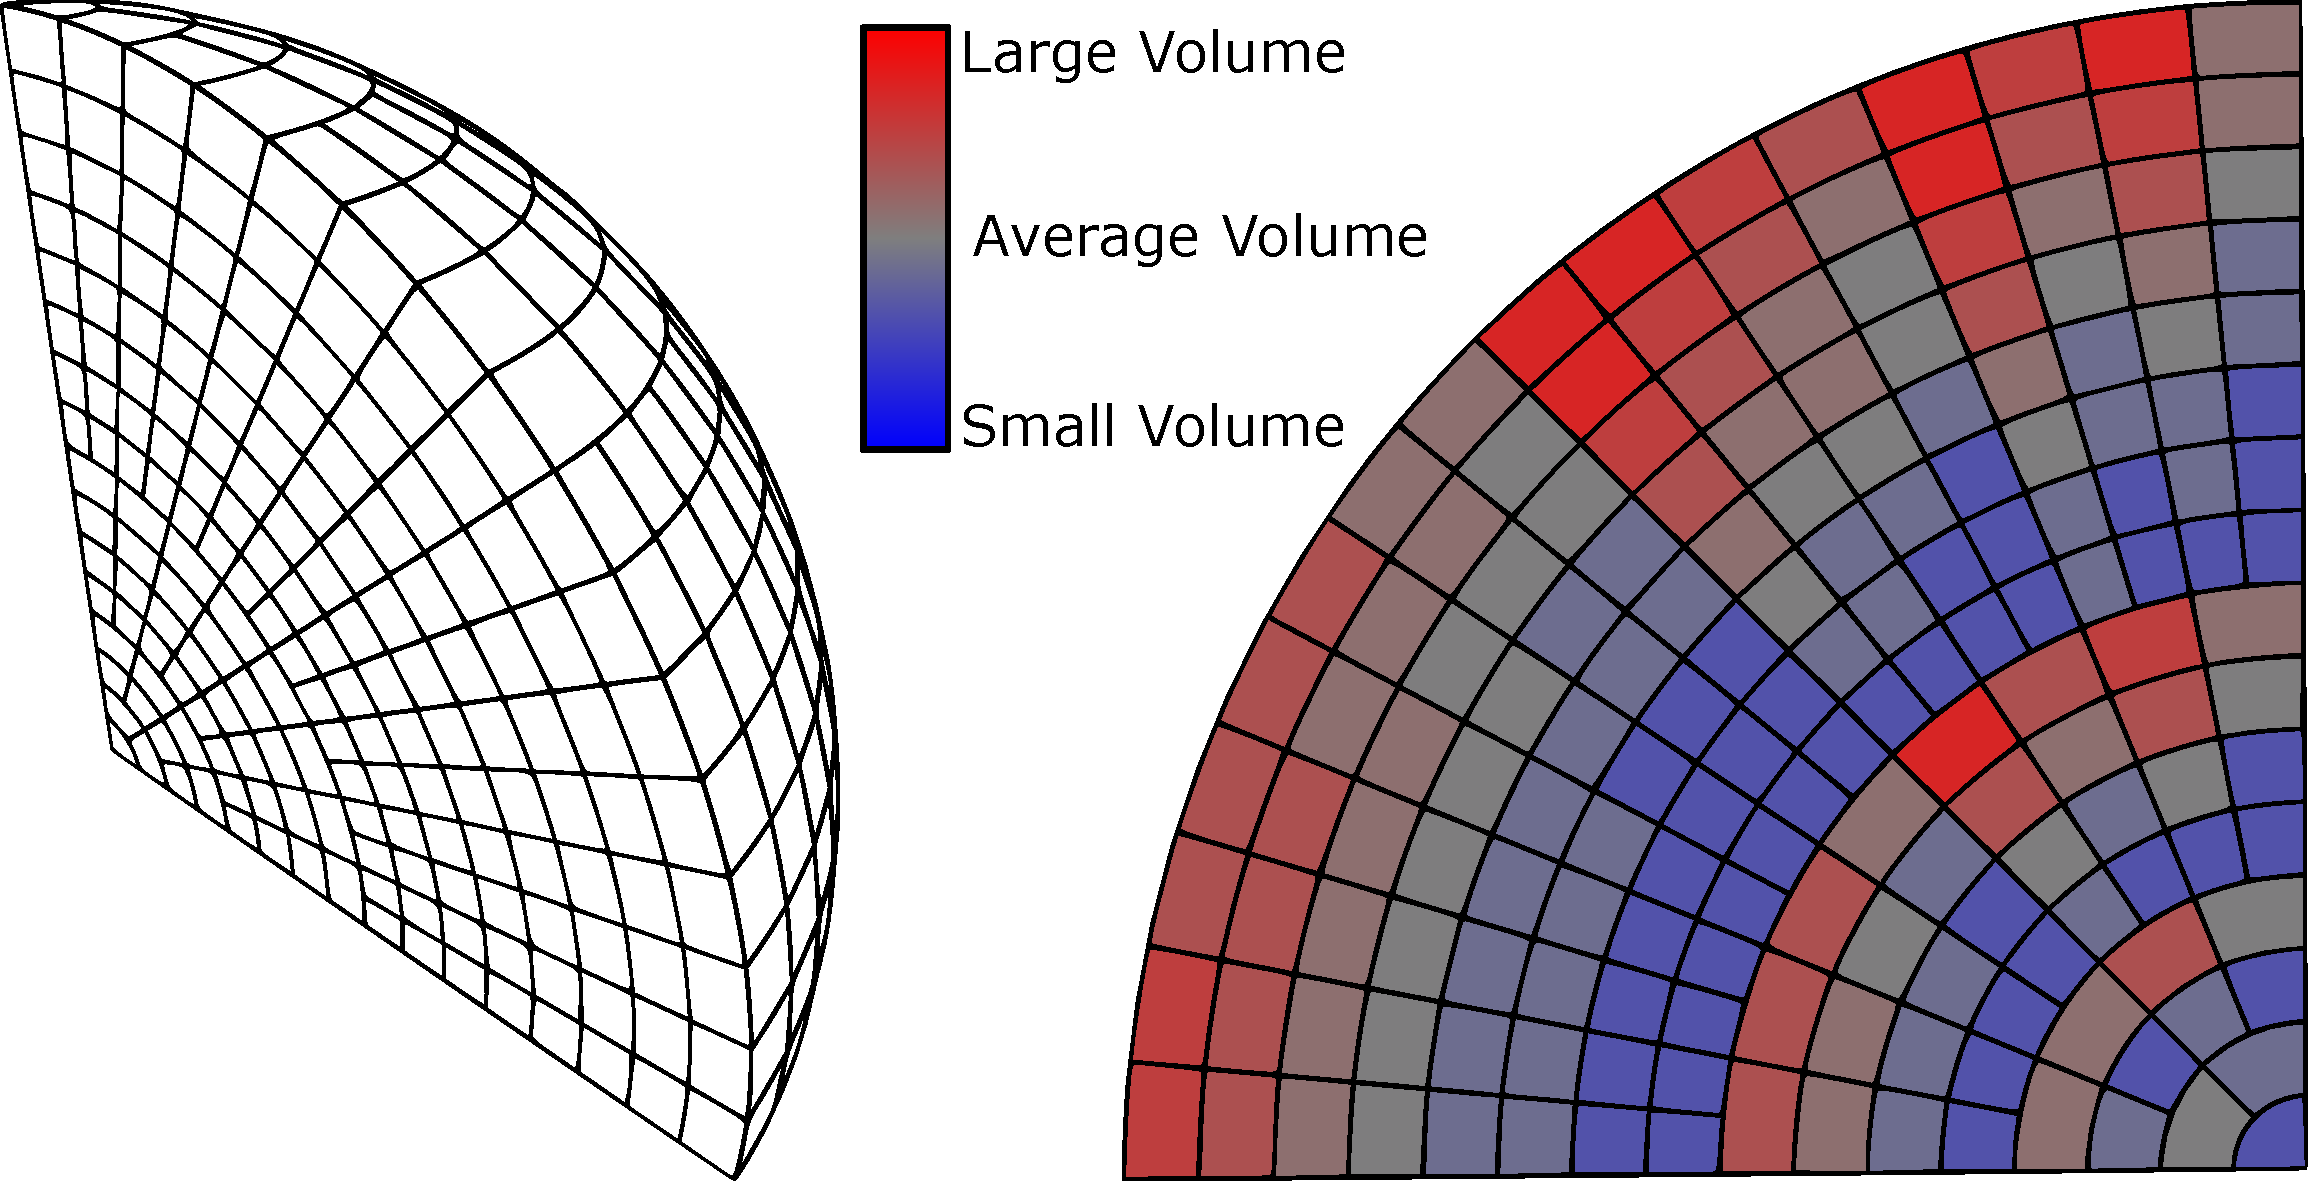
\includegraphics[width=0.85\textwidth]{sdog-volume.pdf}
	\caption[Title]{
		Distribution of cell volumes in an octant after four levels of conventional SDOG refinement
	}
	\label{fig:sdog-volume}
\end{figure}


\begin{figure}[ht!]
	\centering
	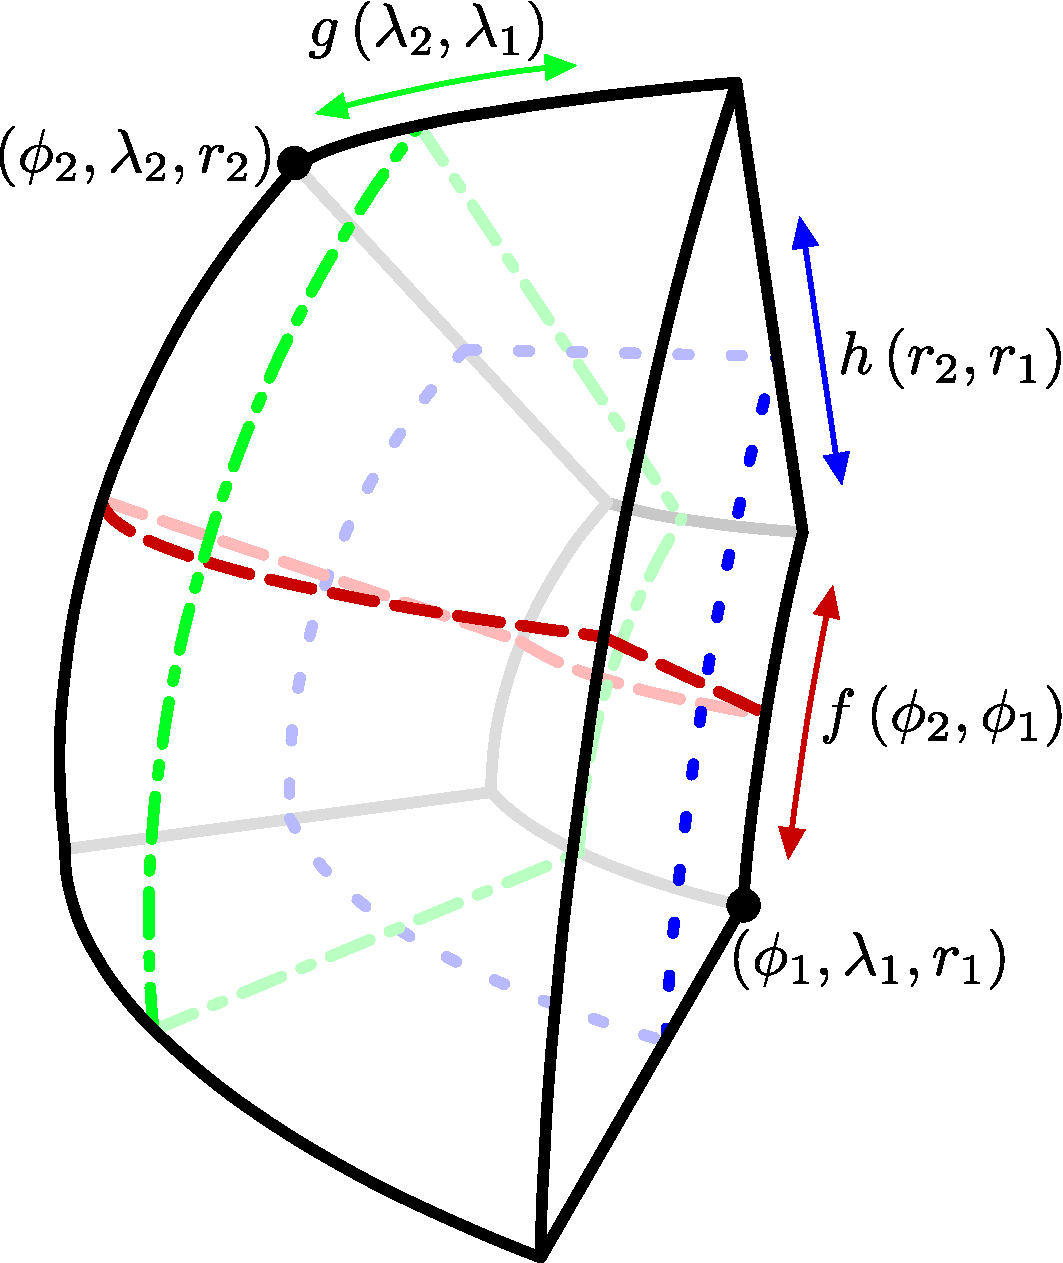
\includegraphics[width=0.4\textwidth]{sdog-functions.pdf}
	\caption[Title]{
		Each SDGO cell represents a range in each spherical coordinate; the location of the splitting surfaces are expressed as a function of the maximum and minimum of the respective range.
		Here we show only an NG cell; however, the same applies to SG and LG cells.
		The functions $f$, $g$, and $h$ serve as placeholders for any valid function that results in the output being strictly between the two inputs
	}
	\label{fig:functions}
\end{figure}


By allowing the location of the splitting surfaces to be adjusted, we can modify the shape and size of child cells and as a result affect the volume preservation, compactness, and other properties of the grid.
Let $c_{s}$ be the location of the splitting surface, where $c$ is one of $\left\lbrace \phi, \lambda, r \right\rbrace$.
One way to express the location of the splitting surfaces used for refinement is as a convex combination of maximum and minimum values:
%
\begin{equation*}
c_{s} = \alpha c_\mathrm{max} + \left( 1-\alpha \right) c_\mathrm{min}, \quad \alpha \in \left( 0, 1 \right),
\end{equation*}
%
where we call $\alpha$ the splitting factor.
Conventional SDOG used midpoints (i.e. $\alpha = 1/2$) for each spherical coordinate during refinement, regardless of cell type.
While a convex combination is the most straightforward, any function of the maximum and minimum such that the result is strictly between the two is a valid method for determining the location of the splitting surfaces (Figure~\ref{fig:functions}).
Thus, the location of splitting surfaces is modified by changing this function, either by using a different value of $\alpha$ or by using a different function altogether.
Furthermore, the function used can be different for each cell type and spherical coordinate.


A useful function for improving volume preservation is one that results in one of the new ranges having a specific percentage of the volume of the original range.
We start with the radial splitting surface.
Referring to Equation~(\ref{eq:volume}), let $p \in (0,1)$ be the percentage we wish for the lower range to have, then
%
\begin{equation*}
p \left( r_\mathrm{max}^{3} - r_\mathrm{min}^{3} \right) = r_{s}^{3} - r_\mathrm{min}^{3}
\end{equation*}
%
\begin{equation*}
p r_\mathrm{max}^{3} - p r_\mathrm{min}^{3} = r_{s}^{3} - r_\mathrm{min}^{3}
\end{equation*}
%
\begin{equation*}
r_{s}^{3} = p r_\mathrm{max}^{3} + r_\mathrm{min}^{3} - p r_\mathrm{min}^{3}
\end{equation*}
%
\begin{equation*}
r_{s}^{3} = p r_\mathrm{max}^{3} + \left( 1 - p \right) r_\mathrm{min}^{3}
\end{equation*}
%
\begin{equation} \label{eq:radVol}
r_{s} = \sqrt[3]{ p r_\mathrm{max}^{3} + \left( 1 - p \right) r_\mathrm{min}^{3} }.
\end{equation}
%
The derivations for the latitudinal and longitudinal splitting surfaces follow the same, with results
%
\begin{equation} \label{eq:latVol}
\phi_{s} = \sin^{-1} \left( p \sin\phi_\mathrm{max} + \left( 1 - p \right) \sin\phi_\mathrm{min} \right) \quad\text{and}
\end{equation}
%
\begin{equation} \label{eq:longVol}
\lambda_{s} = p \lambda_\mathrm{max} + \left( 1 - p \right) \lambda_\mathrm{min}.
\end{equation}


The question then becomes which splitting surfaces should be modified, and in which ways, in order to improve the volume preservation of the grid.
We first look at which splitting surfaces should \textit{not} be modified.
From Equation~(\ref{eq:longVol}), it is clear a longitudinal splitting surface at the midpoint will always split a cell exactly in half, and therefore they should not be changed.


\begin{figure}[ht!]
	\centering
	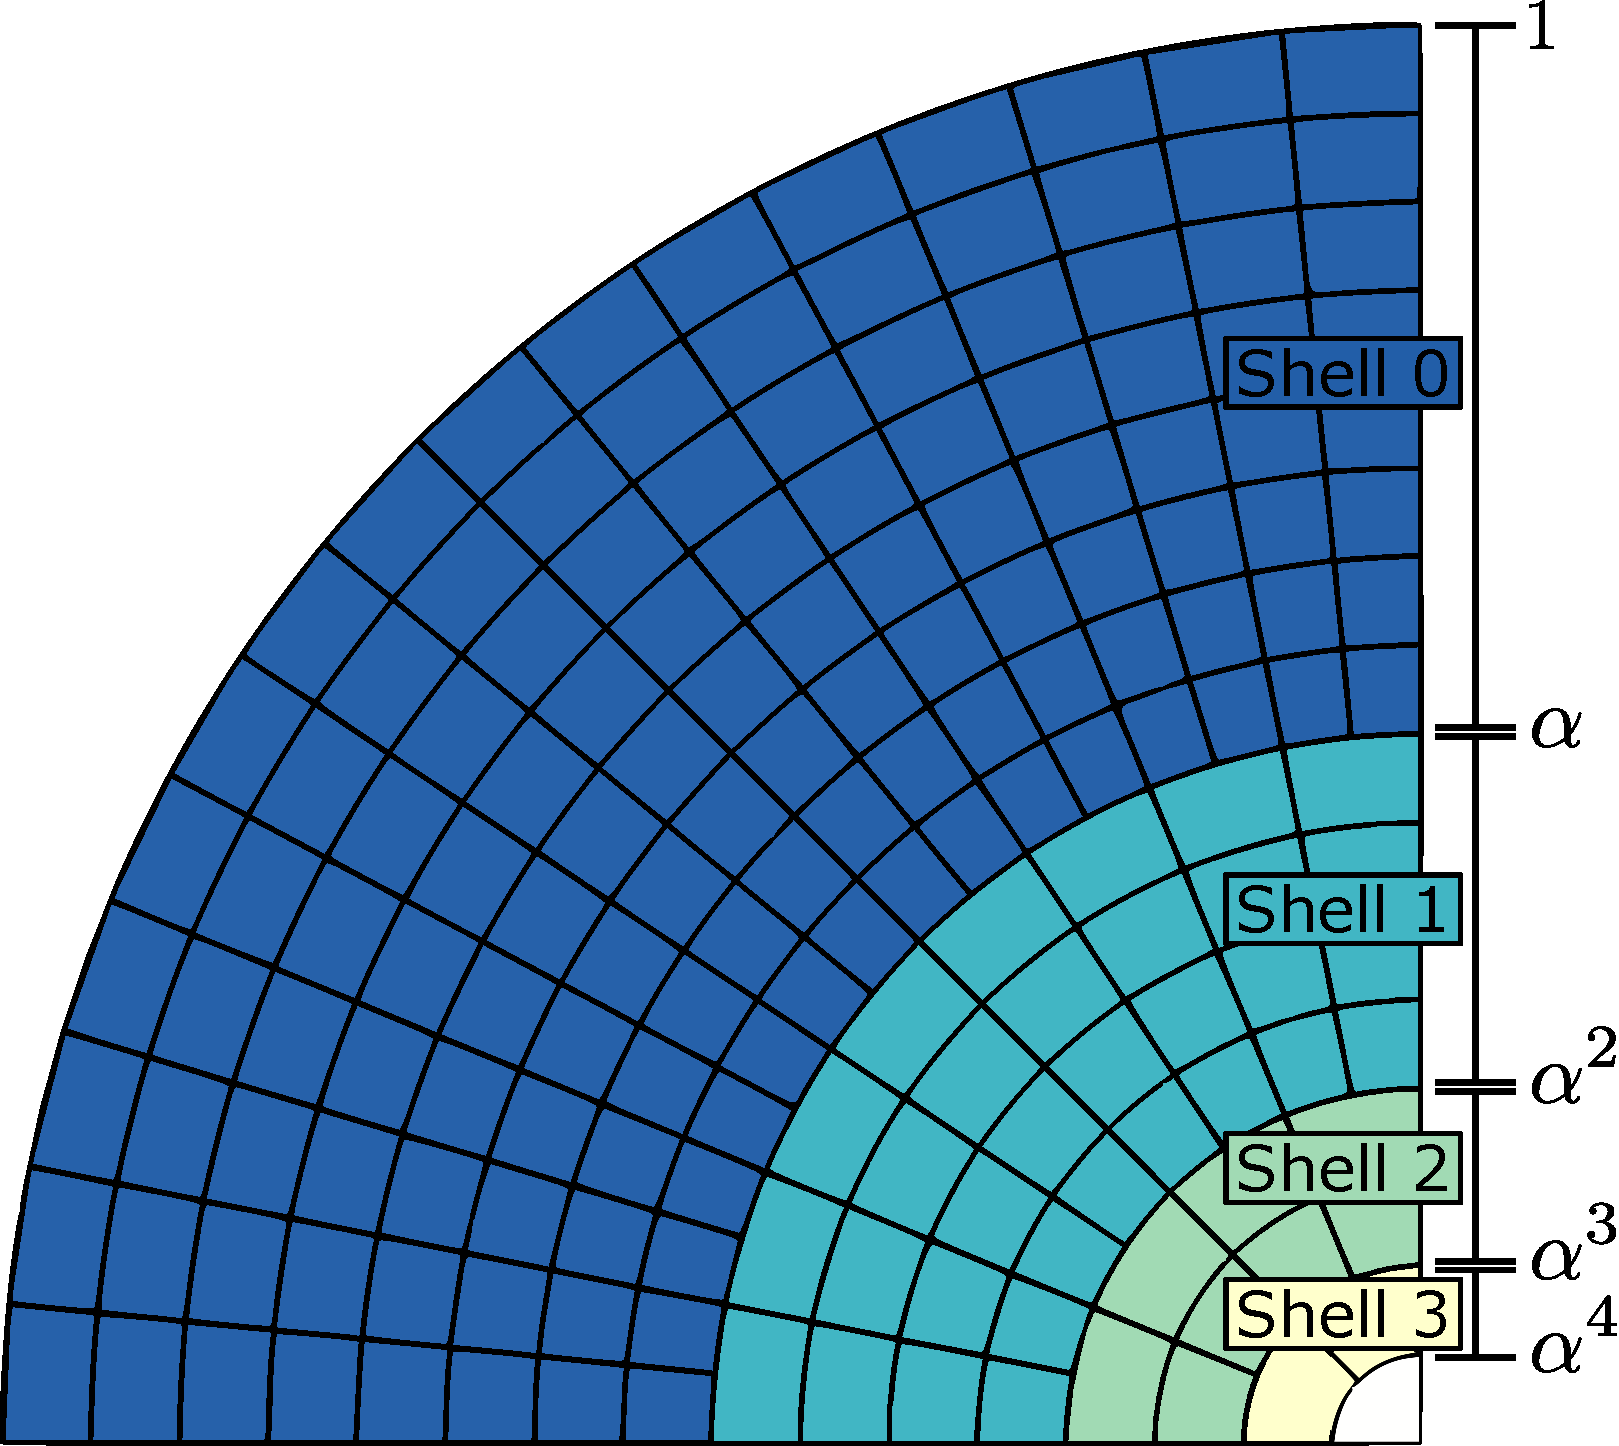
\includegraphics[width=0.6\textwidth]{sdog-shells.pdf}
	\caption[Title]{
		Spherical shells created by the radial splitting surfaces of SG cells.
		At $k$ levels of refinement there are $k$ shells and one inner SG cell.
		These shells are similar and should have volume proportional to the number of cells they contain
	}
	\label{fig:sdog-shells}
\end{figure}


Less trivially, the radial splitting surface for SG cells should also be left at the midpoint.
Referring to Figure~\ref{fig:sdog-shells}, we see that the radial splitting surfaces for SG cells separate the grid into spherical shells.
Shell $n$ has a volume proportional to
%
\begin{equation*}
\alpha^{3n} - \alpha^{3 \left( n + 1 \right)},
\end{equation*}
%
so the ratio of the volumes of shell $n+1$ and $n$ is
%
\begin{equation*}
\frac{ \alpha^{3 \left(n + 1 \right)} - \alpha^{3\left( n + 2 \right)} }{ \alpha^{3n} - \alpha^{3 \left( n + 1 \right)} } = \frac{ \alpha^{3} \alpha^{3n} \left( 1 - \alpha^{3} \right) }{ \alpha^{3n} \left( 1 - \alpha^{3} \right) } = \alpha^{3}.
\end{equation*}
%
From the self similar nature of SDOG refinement, we know that the cells in shell $n$ are simply the cells of shell $n+1$ refined once.
We also know that, in the limit, an SDOG grid at one level higher of refinement will have eight times as many cells as the previous resolution ($\lim_{k \to \infty} T(k+1) / T(k)  = 8 $).
Therefore, in order for cells in the grid to be close to equal volume, it must be that shell $n+1$ has one eighth the volume of shell $n$---since it will have one eighth the number of cells---which occurs exactly when $\alpha = 1 / 2$.


We are left with five possible splitting surfaces to be modified: the radial splitting surface for LG and NG cells, and the latitudinal splitting surface for SG, LG, and NG cells.
Below, we determine the ideal placement for each of these surfaces to maximize volume preservation between cells.
We then propose other possible splitting surface combinations to balance the tradeoff between volume preservation and cell compactness.


\subsection{Ideal Splitting Surfaces for Volume Preservation} \label{chap:4:ideal}
Ideal splitting surfaces to maximize volume preservation are achieved using Equations~(\ref{eq:radVol}) and (\ref{eq:latVol}); all that is required is to determine the ideal value of $p$ for the different splitting surfaces and cell types.
We start with the radial splitting surfaces for LG and NG cells, and the latitudinal one for NG cells, as these surfaces behave the same as regular refinement.
Specifically, these splitting surfaces result in the same number and type of cells on both sides, a property that also holds for their children.
We call these the regular splitting surfaces.
Therefore, we require that the volume on each side of the regular splitting surfaces be equal, or in other words, we set $p = 1/2$ for these splitting surfaces.


\begin{figure}[ht!]
	\centering
	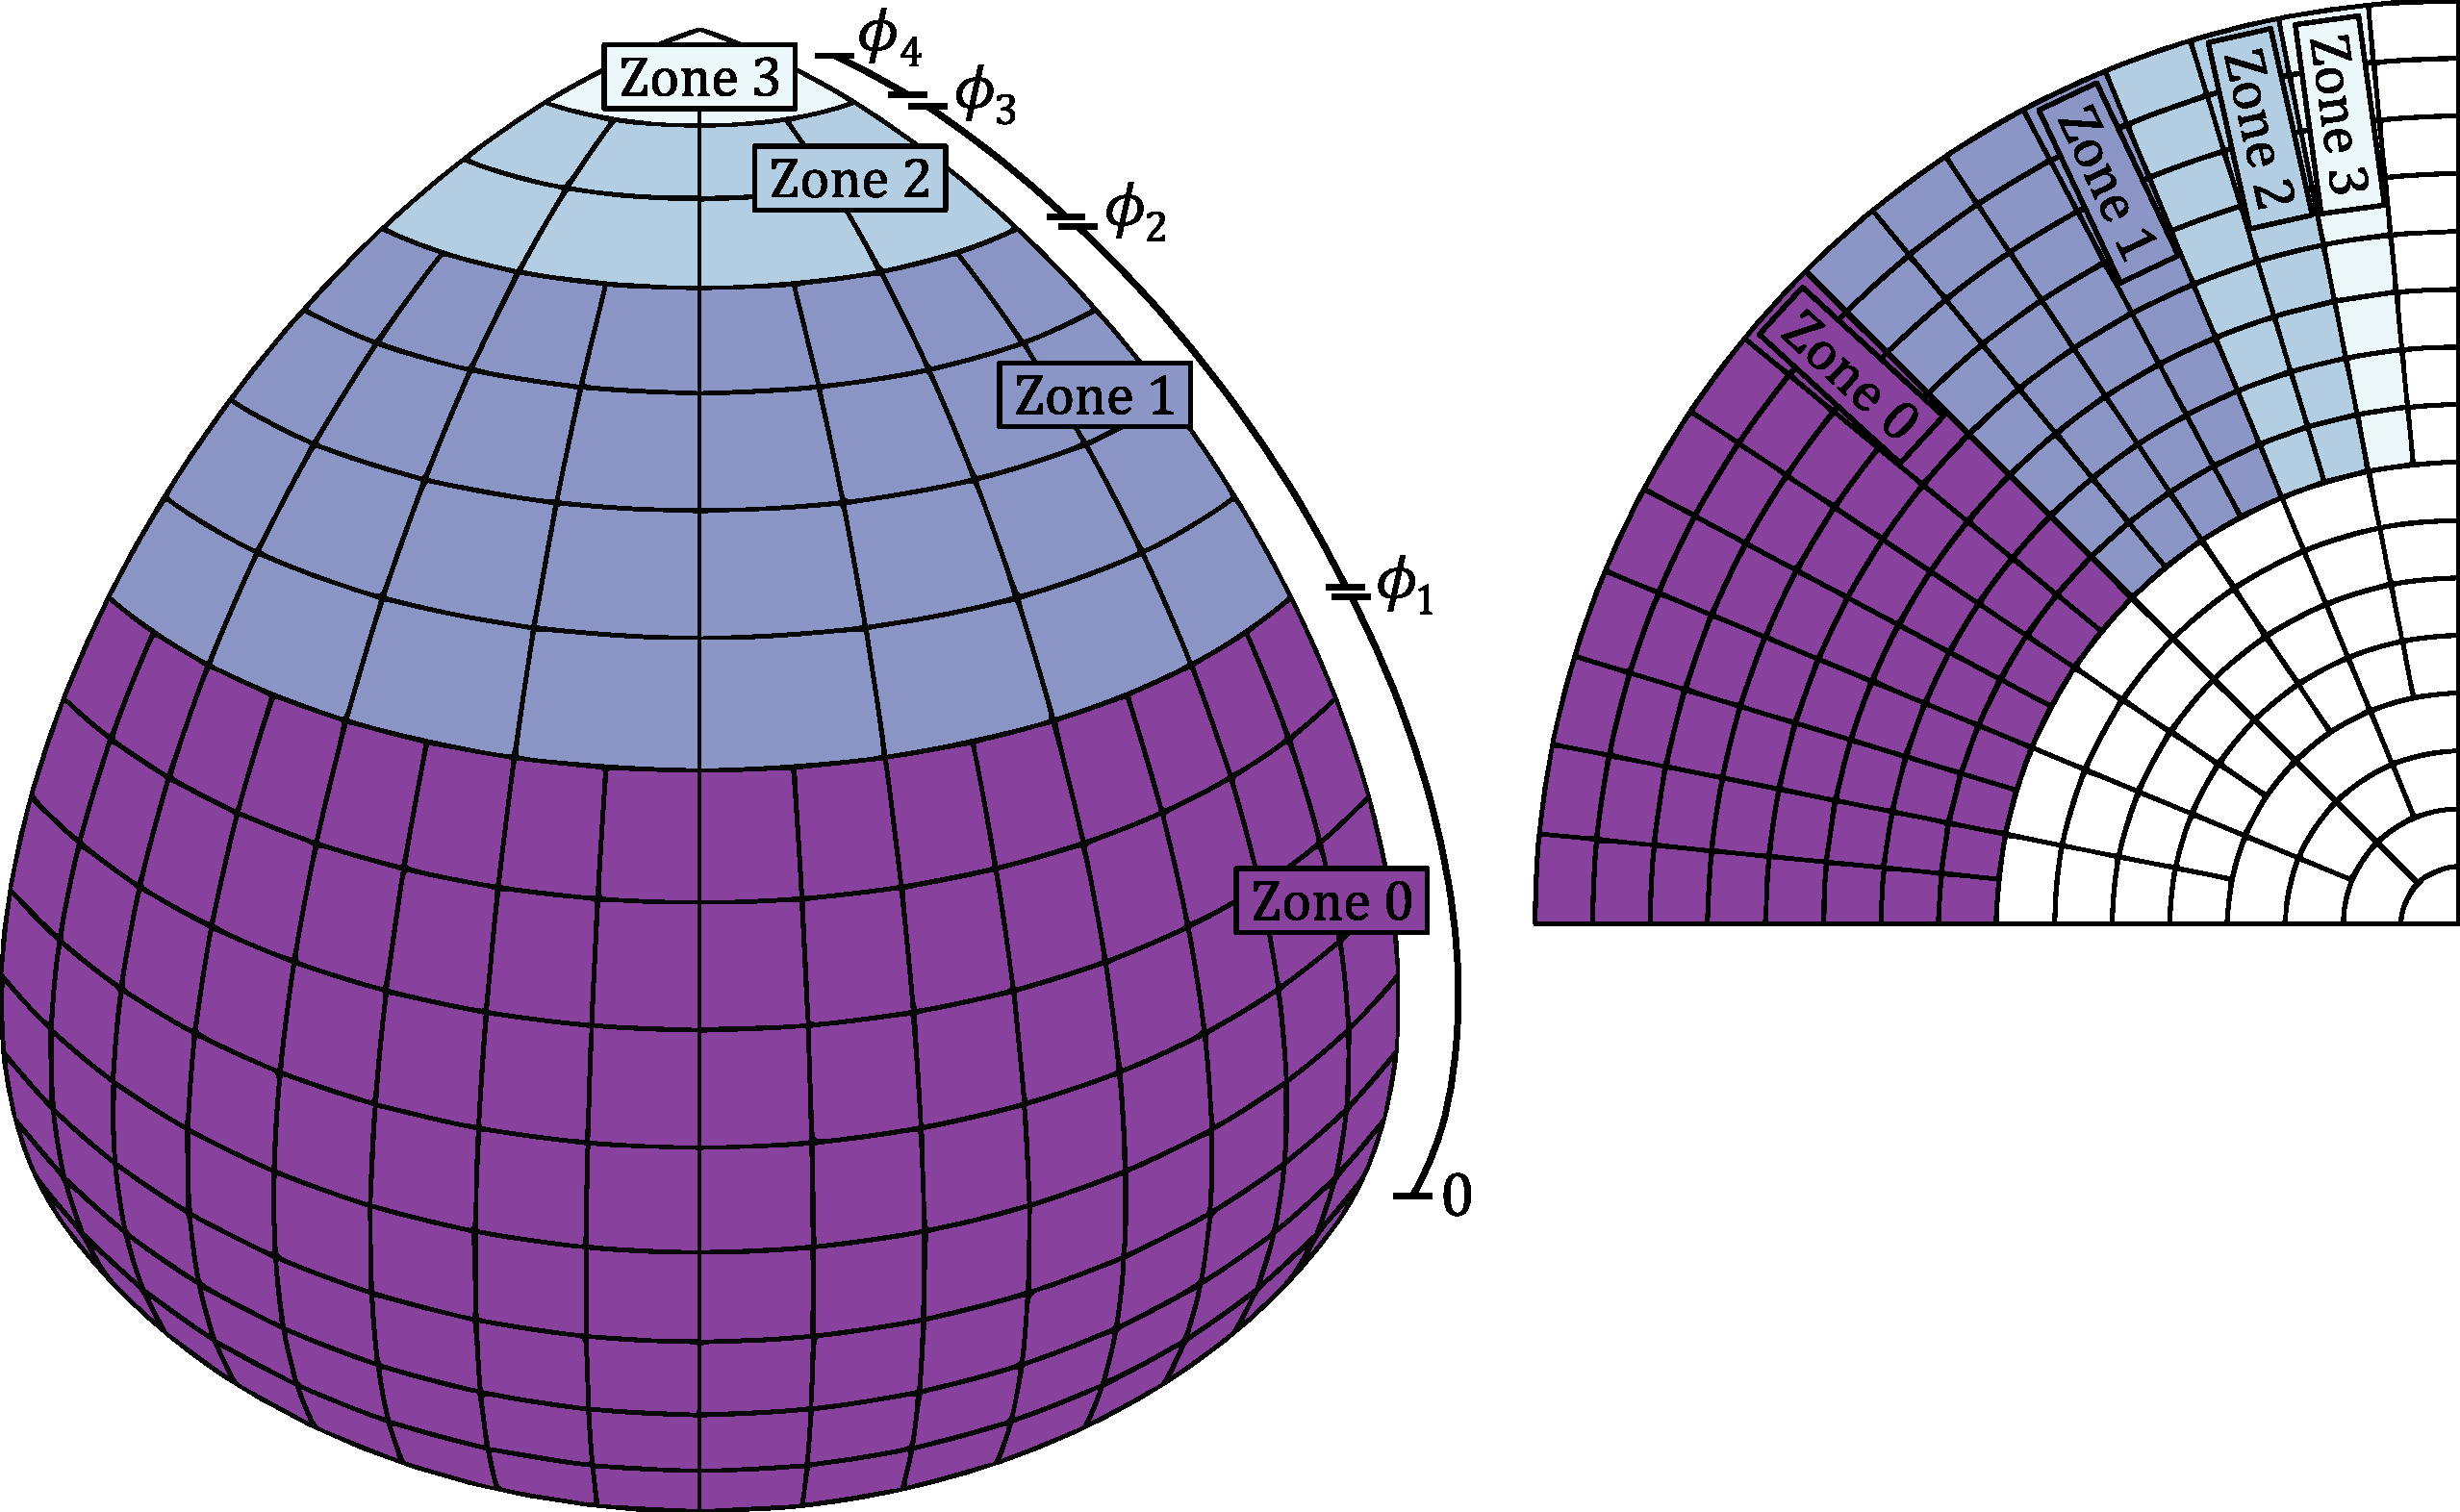
\includegraphics[width=0.9859\textwidth]{sdog-zones.pdf}
	\caption[Title]{
		Spherical zones created by the latitudinal splitting surfaces of SG and LG cells.
		At $k$ levels of refinement, there are $k$ zones and one upper stack of LG cells in the outermost shell.
		Each successively smaller shell has one fewer zone than the previous until reaching the innermost SG cell.
		Zones in the same shell are not exactly similar, but are regular grid regions and should have volume proportional to the number of cells they contain
	}
	\label{fig:sdog-zones}
\end{figure}


Determining the ideal latitudinal splitting surfaces for SG and LG cells is more involved.
First, notice that these two latitudinal splitting surfaces have a similar effect as the radial splitting surface for SG cells.
Referring to Figure~\ref{fig:sdog-zones}, we see that these splitting surfaces further divide the spherical shells into spherical zones.
Additionally, each zone is comprised entirely of NG cells.
From this, we conclude that zone $n$ has precisely four times as many cells as zone $n+1$, and thus, should have four times the volume as well.
Using this information, we find the value for $p$.
Zone $n$ has a volume equal to $\left( 1 - p \right)^{n} p$ that of the initial octant, then setting the ratio between zone $n+1$ and $n$ to be equal to $1/4$ gives us $p = 3/4$.


\begin{figure}[ht!]
	\centering
	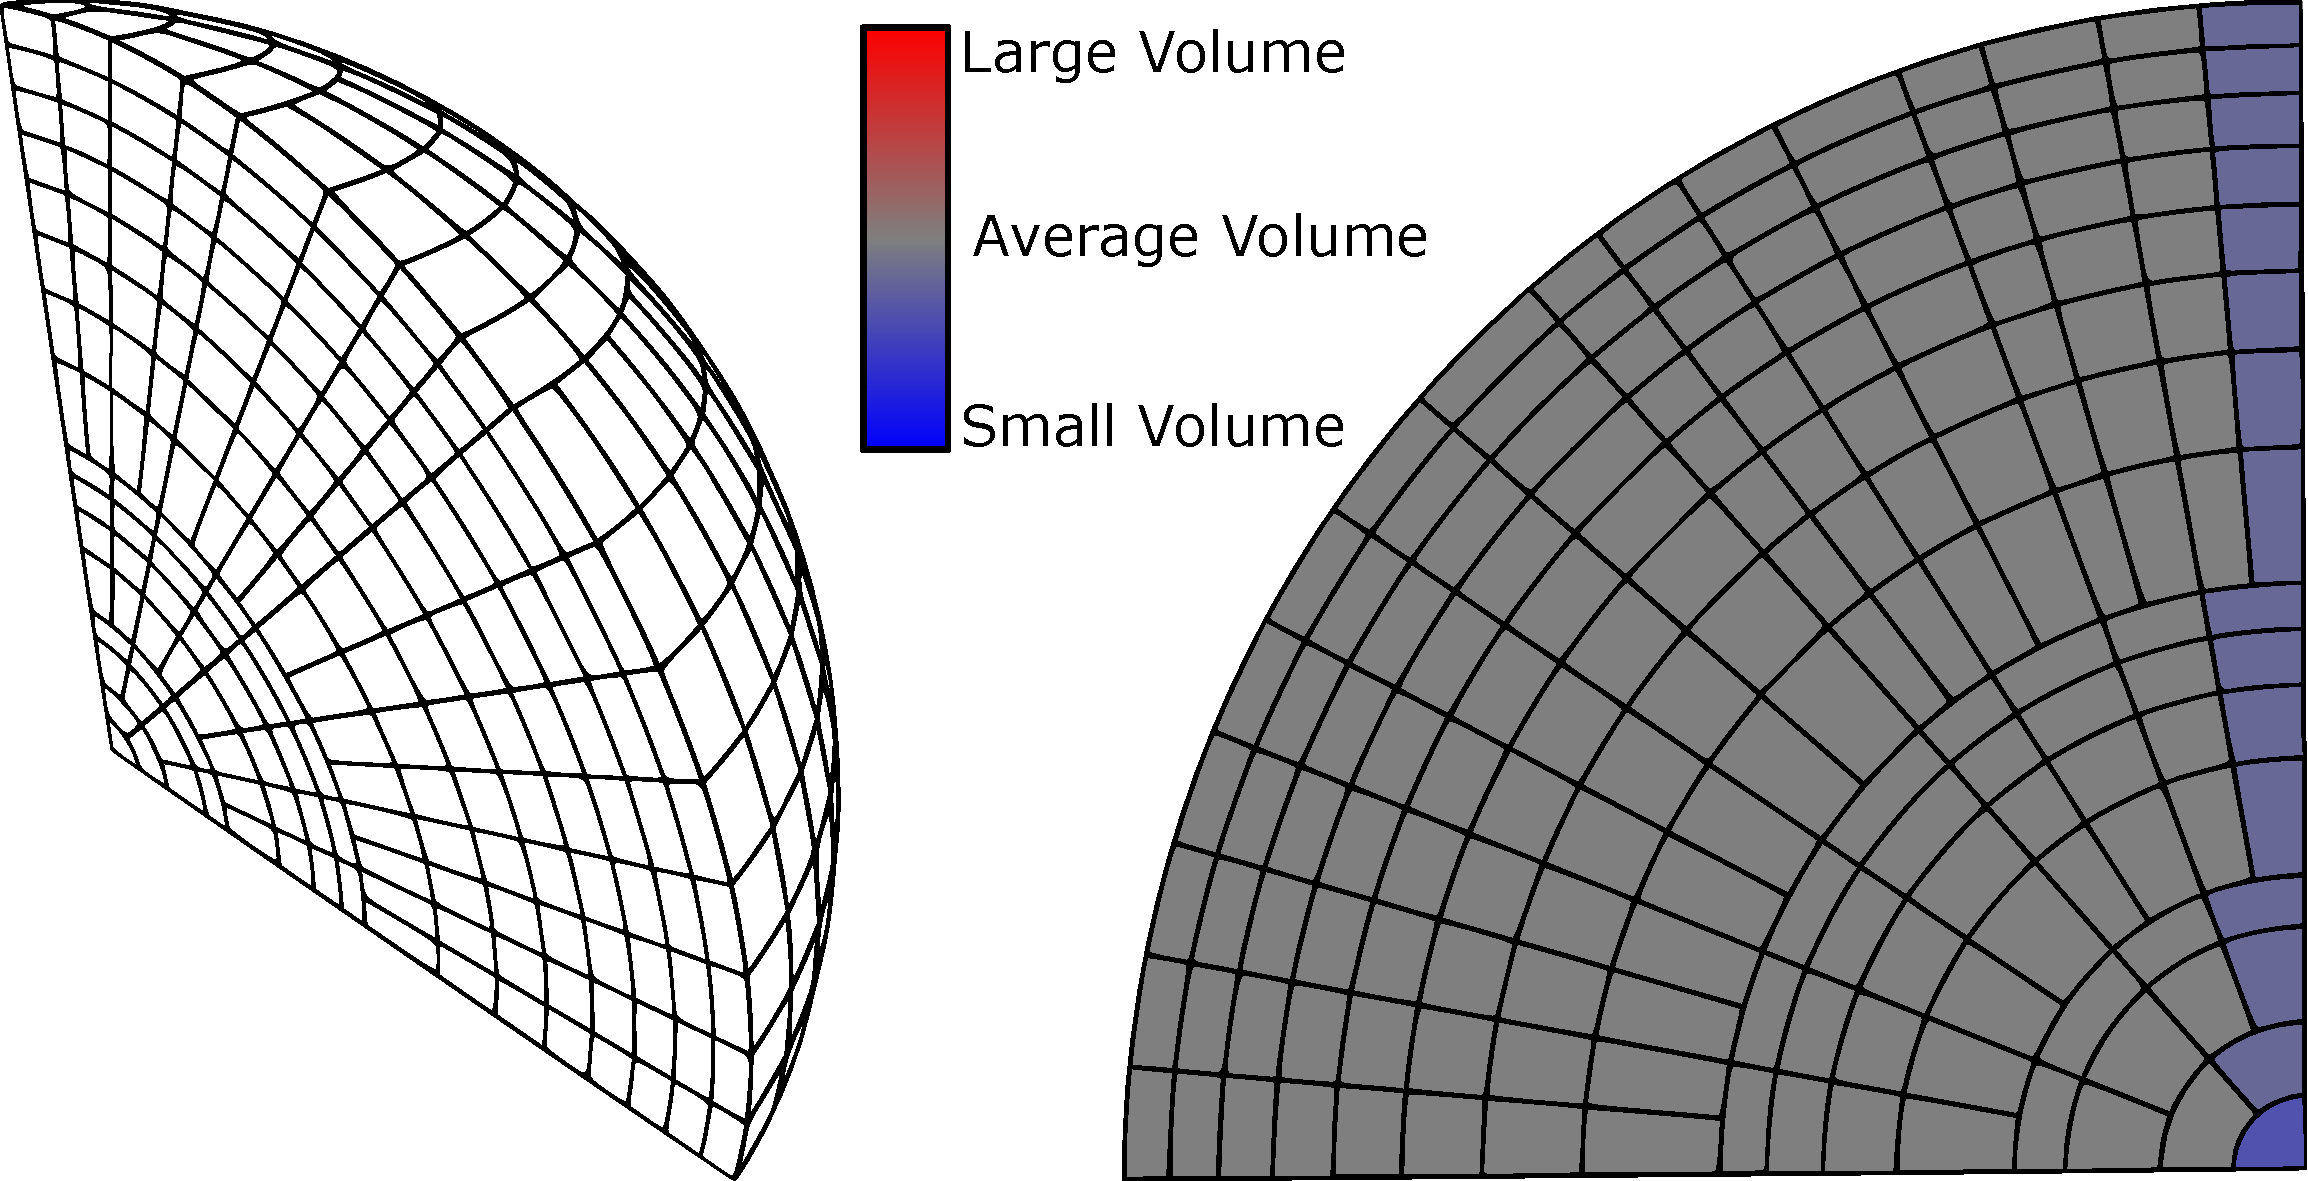
\includegraphics[width=0.85\textwidth]{modified-volume.pdf}
	\caption[Title]{
		Results of the volume method after four levels of refinement.
		All NG cells have exactly the same volume, with the LG and SG cells having a lower volume.
		Notice how the resulting NG cells are stretched and squashed in order to ensure they all have equal volume
	}
	\label{fig:modified-volume}
\end{figure}


Figure~\ref{fig:modified-volume} shows the resulting grid from this method of calculating splitting surfaces, which we refer to as the \textit{volume} method.
In this grid, all NG cells at the same level of refinement have equal volume; this dramatically improves the volume preservation, as only cells that extend to one of the singularities (i.e. SG and LG cells) will have a different volume than the other cells in the grid.


\subsection{Balanced Splitting Surfaces} \label{chap:4:balanced}
While the above refinement method significantly improves volume preservation in the grid, this gain does not come without consequence.
Cells are stretched and squashed in order to achieve this volume preservation, which reduces cell compactness and may be an undesirable effect depending on the application.
In order to address this issue, it is possible to use different splitting surfaces that achieve a better balance between volume preservation and cell compactness.


\begin{figure}[ht!]
	\centering
	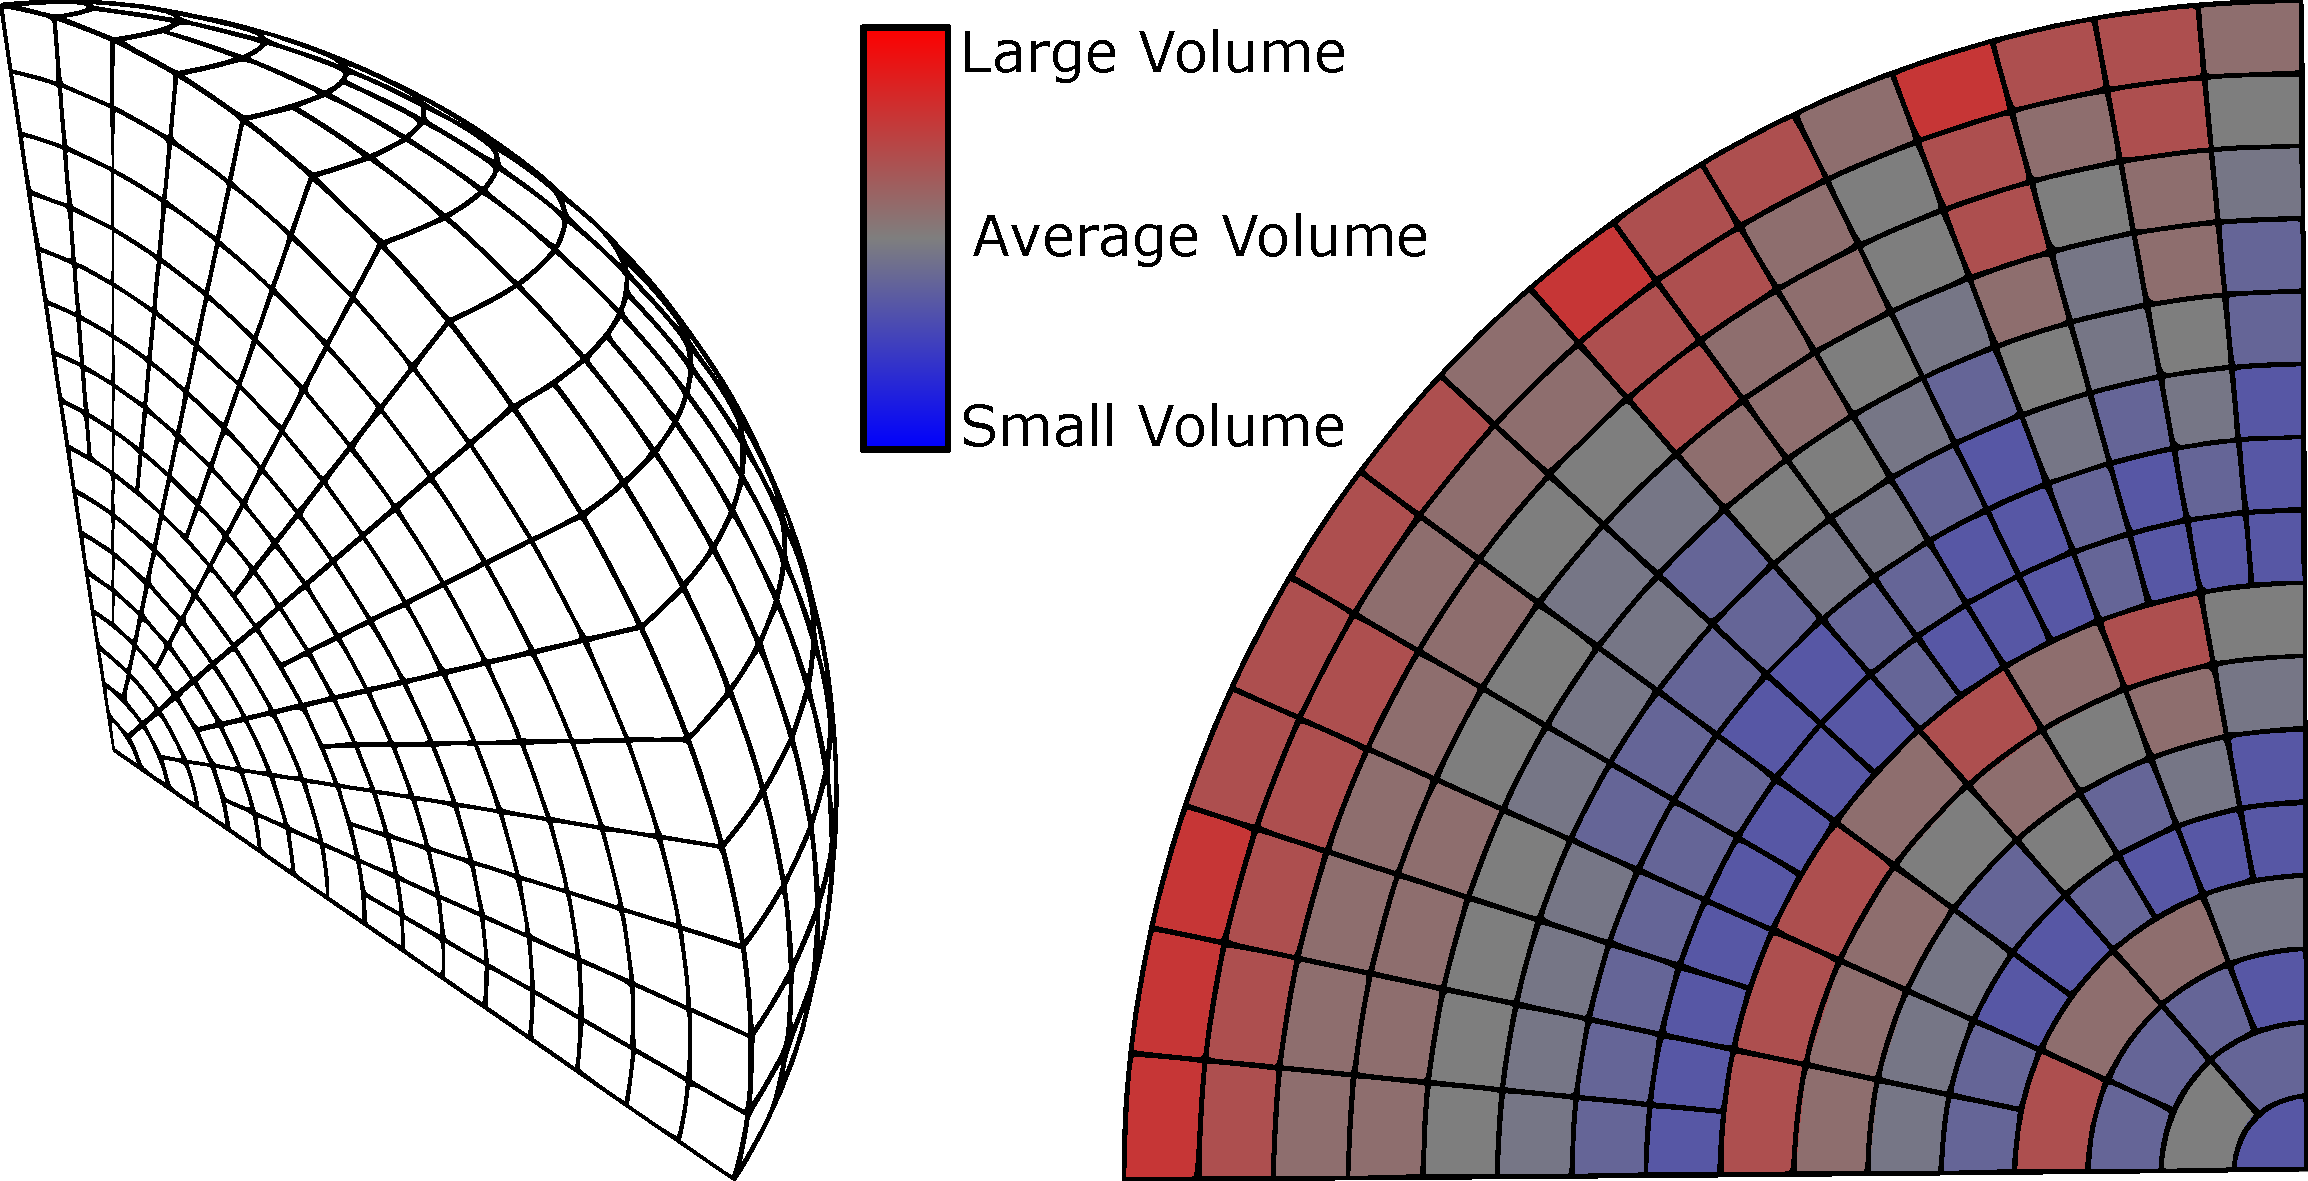
\includegraphics[width=0.85\textwidth]{alpha-volume.pdf}
	\caption[Title]{
		Results of the latitude method after four levels of refinement.
		Since only latitude splitting surface for SG and LG cells have been modified, the results are similar to that of conventional SDOG
	}
	\label{fig:alpha-volume}
\end{figure}


Looking at Figure~\ref{fig:modified-volume}, we see that the regular splitting surfaces are responsible for the majority of the reduction in cell compactness.
Our first balanced scheme then is to leave these splitting surfaces at the midpoints and only modify the latitudinal splitting surfaces for SG and LG cells.
Figure~\ref{fig:alpha-volume} shows the results of this method, which we refer to as the \textit{latitude} method.
Comparing this to conventional SDOG (refer back to Figure~\ref{fig:sdog-volume}), the two grids are nearly identical.
Thus, this method offers only a slight improvement with regards to volume preservation, while also only slightly sacrificing cell compactness.


\begin{figure}[ht!]
	\centering
	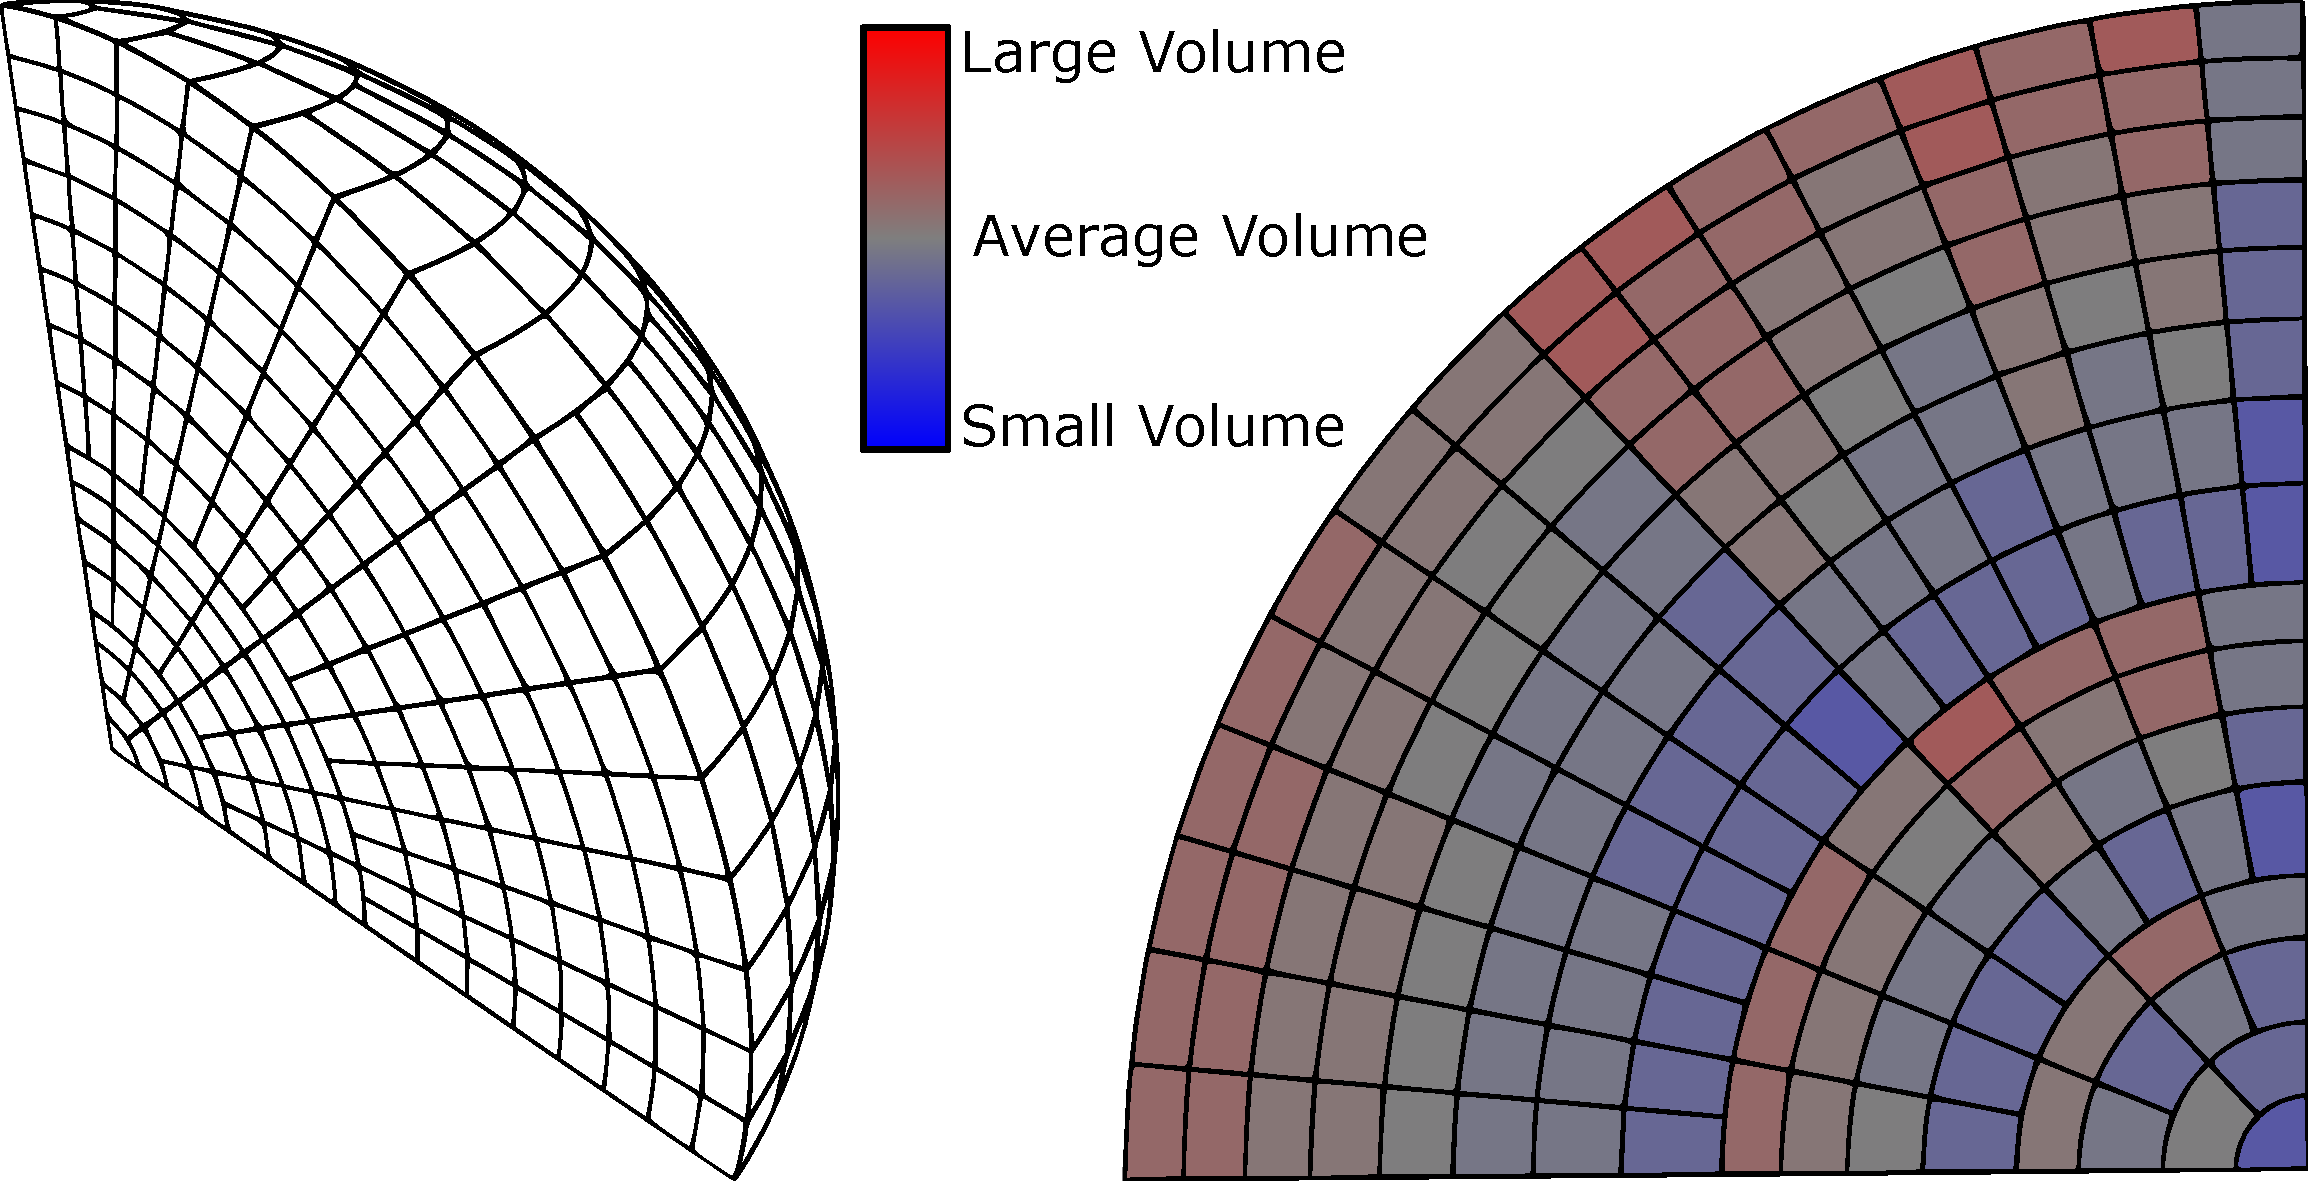
\includegraphics[width=0.85\textwidth]{blend-volume.pdf}
	\caption[Title]{
		Results of the balanced method after four levels of refinement.
		NG cells are still stretched and squashed in order to better preserve volume; however, the effect is less pronounced than in the volume method
	}
	\label{fig:blend-volume}
\end{figure}


In order to achieve different tradeoffs between compactness and volume preservation, modifying the regular splitting surfaces is necessary.
Equations~(\ref{eq:radVol}) and (\ref{eq:latVol}) give ideal placements for volume preservation as compared to the conventional midpoint functions which result in better compactness.
Therefore, using different functions that blend between these two extremes allows for a more balanced tradeoff.
There are endless possibilities for these functions; however, as will be required in Chapter~\ref{chap:mapping}, they should be easily invertible.
That is, given a splitting surface, we need to be able to determine the corresponding value of $p$.
For the radial splitting surfaces, we propose the function
%
\begin{equation*}
r_{s} = \sqrt[t]{ p r_\mathrm{max}^{t} + \left( 1 - p \right) r_\mathrm{min}^{t} }
\end{equation*}
%
where $1 \leq t \leq 3$ blends between compactness at $t = 1$ (equivalent to midpoint) and volume preservation at $t=3$ (equivalent to Equation~(\ref{eq:radVol})).
For the latitudinal splitting surfaces, we propose
%
\begin{equation*}
\phi_{s} = h \sin^{-1} \left( p \sin \left( \frac{1}{h} \phi_\mathrm{max} \right) + \left( 1 - p \right) \sin \left( \frac{1}{h} \phi_\mathrm{min} \right) \right)
\end{equation*}
%
where $1 \leq h \leq \infty$ blends between volume preservation at $h = 1$ (equivalent to Equation~(\ref{eq:latVol})) and compactness at $h = \infty$ (equivalent to midpoint). We found values of $t = 2$ and $h = 1.5$ to offer a relatively balanced tradeoff between the two properties, with the resulting grid shown in Figure~\ref{fig:blend-volume}.
We refer to this method as the \textit{balanced} one.


\section{Results} \label{chap:4:results}
There are several potential methods for evaluating the volume-preserving properties of a 3D DGGS.
When first proposed by Yu and Wu, the ratio between cells of the largest and smallest volume was used to evaluate the volume-preserving properties of SDOG~\cite{yu2009sdog}.
This volume ratio is a useful measure for determining the worst-case difference in the volume of cells; however, it does not give any information about the distribution of said volumes.
For example, a grid with all cells except one having equal volume, and a grid where every cell has a distinct volume, could end up having the same volume ratio.
To get a complete understanding of volume preservation, we should also examine statistics that give a measure of distribution.
For this purpose, we use the coefficient of variation (CV), which is simply the ratio between the standard deviation (SD) and the mean.
We use the CV over the SD as it a dimensionless quantity.


\begin{figure}[htp!]
	\centering
	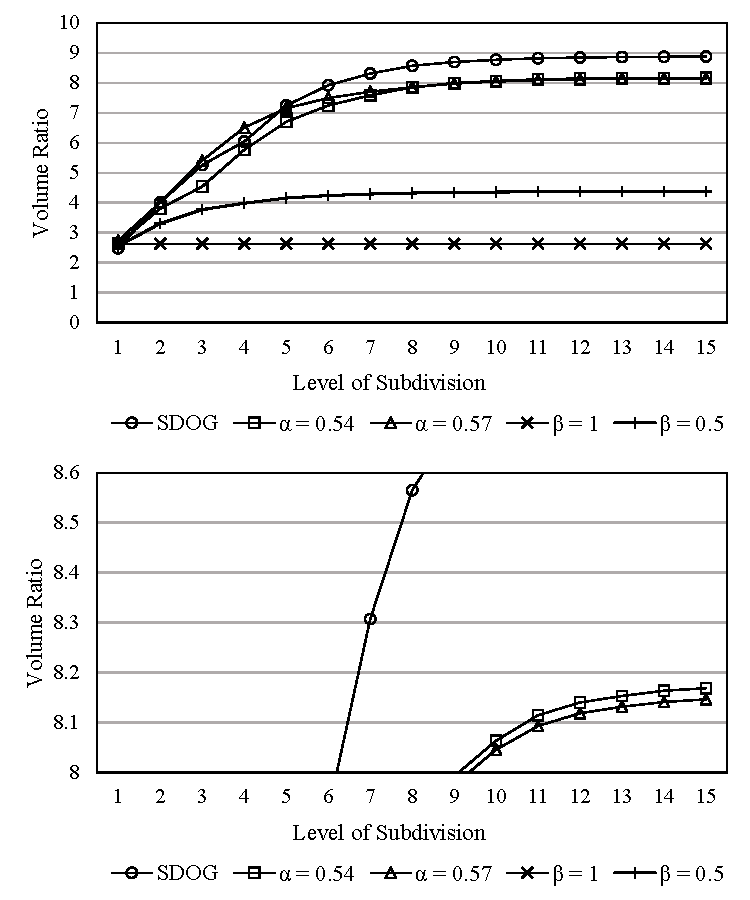
\includegraphics[width=0.75\textwidth]{volume-ratio.pdf}
	\caption[Title]{
		Volume ratio for the different grids at increasing levels of refinement.
		Note that for the non-stationary method ($\beta = 1$) the volume ratio does not change with refinement level
	}
	\label{fig:vr}
\end{figure}



\begin{figure}[htp!]
	\centering
	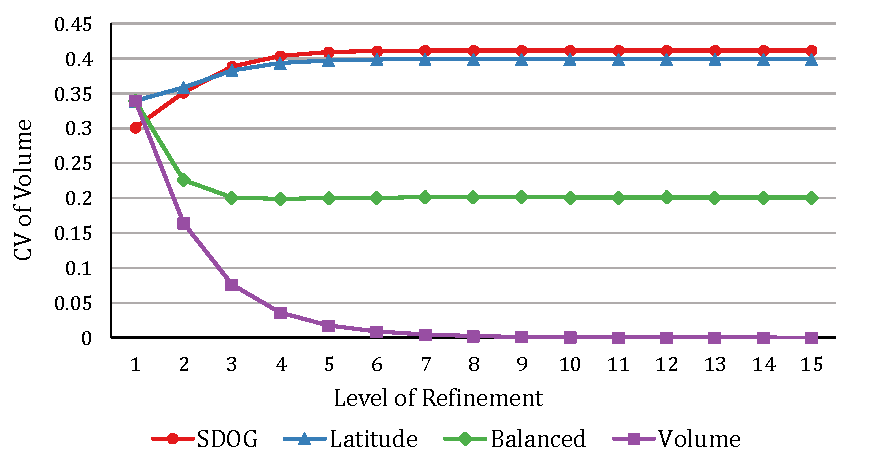
\includegraphics[width=0.75\textwidth]{cv-volume.pdf}
	\caption[Title]{
		CV of volume for the different grids at increasing levels of refinement
	}
	\label{fig:cv}
\end{figure}


In modifying the refinement for volume preservation, it is also important to evaluate the impact these changes have on other properties of the grid.
Specifically, we should measure the effect our changes have on the compactness of cells.
To measure this, we use the notion of sphericity, which quantifies how closely the shape of an object approximates a sphere~\cite{wadell1935volume}.
Sphericity is defined as the ratio between the surface area of a sphere with the same volume as the object and the surface area of the object itself.
Therefore, a perfect sphere will have a sphericity of one, and any other object will have sphericity strictly less than one.
Formally, given an object $\omega$ and a sphere $s$ such that $\operatorname{vol}(s) = \operatorname{vol}(\omega)$, the sphericity of $\omega$, $\Psi$, is given by $\operatorname{area}(s) / \operatorname{area}(\omega)$ , or equivalently 
%
\begin{equation*}
\Psi = \frac{\pi^{\frac{1}{3}}\left( 6\operatorname{vol}(\omega) \right)^{\frac{2}{3}}}{\operatorname{area}(\omega)}.
\end{equation*}
%
We use the mean and SD of sphericity for all cells in the grid to evaluate compactness globally.


\begin{figure}[htp!]
	\centering
	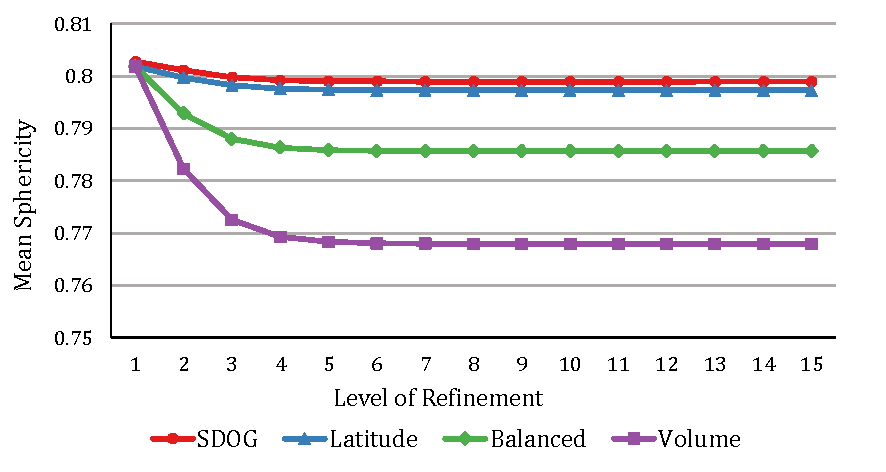
\includegraphics[width=0.75\textwidth]{mean-sph.pdf}
	\caption[Title]{
		Mean sphericity for the different grids at increasing levels of refinement
	}
	\label{fig:sph}
\end{figure}


\begin{figure}[htp!]
	\centering
	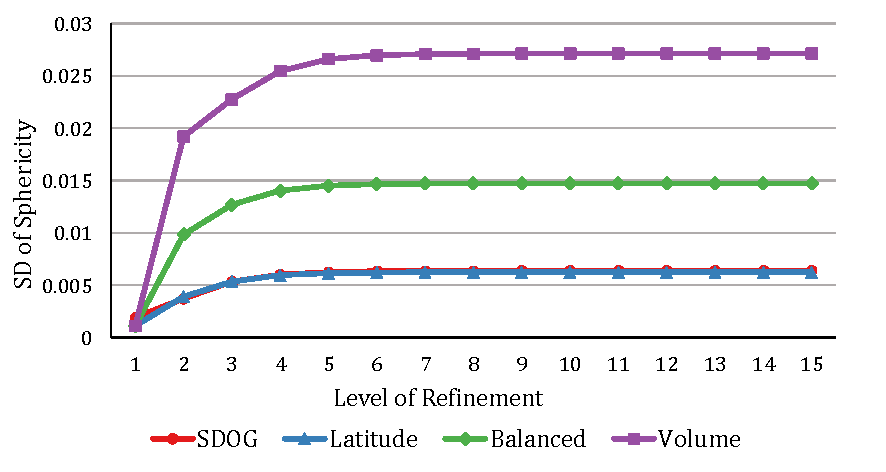
\includegraphics[width=0.75\textwidth]{sd-sph.pdf}
	\caption[Title]{
		Standard deviation of sphericity for the different grids at increasing levels of refinement
	}
	\label{fig:sd-sph}
\end{figure}


As a baseline, we have calculated the value of these measures at each refinement level from one to fifteen for conventional SDOG.
We then repeated this for the three modifications discussed in this chapter: the volume method, the latitude method, and the balanced method.
The results for each grid are displayed in Figures~\ref{fig:vr}, \ref{fig:cv}, \ref{fig:sph}, and \ref{fig:sd-sph} showing the volume ratio, CV of volume, mean sphericity, and SD of sphericity, respectively.
Table~\ref{tab:results} summarizes these charts with the convergence value of each property for the four different grids.
We also give convergence values for the maximum and minimum sphericity---and their difference---for each grid in Table~\ref{tab:results-sph}.
It is important to note that for volume ratio and CV of volume, lower values are better, but for mean sphericity, a higher value is better.


\begin{table}[htp!]
	\centering
	\caption[Title]{
		Convergence value of each measure for the four discussed grids
	}
	\begin{tabular}{|c|c|c|c|c|c|}
		\hline
		& SDOG & $\alpha_{\phi}^{SG} \approx 0.54$ & $\alpha_{\phi}^{SG} = 0.57$ & $\beta = 1$ & $\beta = 0.5$ \\ \hline
		Volume Ratio     & 8.88   & 8.17   & 8.15   & 2.63      & 4.37   \\ \hline
		CV of Volume     & 0.412  & 0.399  & 0.409  & 6.44E-19  & 0.211  \\ \hline
		Mean Sphericity  & 0.799  & 0.797  & 0.795  & 0.767     & 0.787  \\ \hline
		SD of Sphericity & 0.00639& 0.00629& 0.00727& 0.0271    & 0.0141 \\ \hline
	\end{tabular}
	\label{tab:results}
\end{table}


\begin{table}[htp!]
	\centering
	\caption[Title]{
		Convergence value of max and min sphericity for the four discussed grids
	}
	\begin{tabular}{|c|c|c|c|c|c|}
		\hline
		& SDOG & $\alpha_{\phi}^{SG} \approx 0.54$ & $\alpha_{\phi}^{SG} = 0.57$ & $\beta = 1$ & $\beta = 0.5$ \\ \hline
		Max sphericity & 0.806  & 0.806  & 0.806  & 0.806 & 0.806  \\ \hline
		Min sphericity & 0.754  & 0.763  & 0.766  & 0.672 & 0.728  \\ \hline
		Difference     & 0.0520 & 0.0428 & 0.0404 & 0.134 & 0.0780 \\ \hline
	\end{tabular}
	\label{tab:results-sph}
\end{table}

\textbf{Update this with new discussion once results are in}

The stationary scheme with $\alpha_{\phi}^{SG} \approx 0.54$ has a better volume ratio than conventional SDOG for all levels of refinement except the first, and a lower CV of volume for all levels of refinement after the second.
Comparing this to the one with $\alpha_{\phi}^{SG} = 0.57$, both the volume ratio and CV of volume do not improve as compared to conventional SDOG until the fifth level of refinement.
Both of these methods also reduce the mean sphericity of cells at all levels of refinement, with $\alpha_{\phi}^{SG} = 0.57$ having more than twice the absolute reduction of $\alpha_{\phi}^{SG} \approx 0.54$.
The variation in sphericity is similar between all three of these grids.
Using $\alpha_{\phi}^{SG} = 0.57$ does give a slightly better volume ratio than $\alpha_{\phi}^{SG} \approx 0.54$ as the level of refinement gets large, however this difference is quite small and likely not worth the lower cell compactness and higher variation in volume.


The non-stationary scheme gives a much larger improvement to both the volume ratio and the CV of volume.
This is to be expected, as all NG cells in this scheme have exactly equal volume.
As the level of refinement gets large, the CV of volume quickly approaches zero since the number of NG cells is much larger than the number of LG and SG cells in the grid.
The cost of this improved volume preservation is a much larger reduction in the sphericity of cells and an increase in the variation of sphericity, which is to be expected.
The blending scheme has results in between that of conventional SDOG and the non-stationary scheme, which was also expected.
The CV of volume, mean sphericity, and SD of sphericity are all near the respective halfway points, whereas the volume ratio still ends up being a significant improvement over conventional SDOG.

\section{Summary}
This chapter presents modifications of conventional SDOG refinement that result in improved volume preservation properties in the resulting grids.
The modifications improve volume preservation as measured by two different metrics, at the cost of reducing cell compactness.
Two blending functions---each defined on a single parameter---enable different balances between volume preservation and compactness.
When used for maximum volume preservation, our method results in all non-degenerate cells in the grid having exactly equal volume.
